\documentclass[10pt,journal,compsoc]{IEEEtran}

\usepackage[nocompress]{cite}
\usepackage{graphicx}
\graphicspath{{../../figures_pdf_vector/}}
\usepackage{amsmath,amssymb}
\usepackage{booktabs}
\usepackage{multirow}
\usepackage{array}
\usepackage{xcolor}
\usepackage{url}
\usepackage{listings}
\lstset{basicstyle=\ttfamily\footnotesize,breaklines=true,columns=fullflexible}

% A figure the replication package has not yet produced. The build fails
% verification (verify_tse.py) while any of these remain.
\newcommand{\PENDING}[1]{\textcolor{red}{\textbf{[PENDING: #1]}}}
\newcommand{\RQ}[1]{\textbf{RQ#1}}

\begin{document}

\title{Boundary-Mutation Testing of Secret Scanners: Defects Shared Across Six Tools, Inherited Through Rule Tables, and Repaired}

% Anonymise this block if the submission is double-anonymous (check the
% TSE ScholarOne instructions before submitting).
\author{Shweta~Mishra%
\IEEEcompsocitemizethanks{\IEEEcompsocthanksitem S. Mishra is an independent researcher, Moradabad, India.\protect\\
E-mail: shweta.mishra.research@gmail.com. ORCID: 0009-0002-8443-1678.}}

\markboth{IEEE Transactions on Software Engineering}%
{Mishra: Boundary-Mutation Testing of Secret Scanners}

\IEEEtitleabstractindextext{%
\begin{abstract}
Secret scanners match credentials with regular expressions and are validated by example: fixtures that place each credential in one canonical position. A rule matches a credential \emph{together with} the text around it, so that position is the variable fixtures hold fixed. Boundary-mutation testing varies it. Credentials are generated from each rule's own expression, embedded in contexts real code uses, and judged against a rule-level oracle. We apply it to six scanners, with 1{,}238 credential types generated from five of their rule tables. Every scanner with a defect owes it to one of two boundary strategies. An explicit terminator allowlist, in Gitleaks, misses a credential followed by `\texttt{)}' for 302 of its 427 types, and Kingfisher inherits the same defect through an imported rule table (436 of 616). An implicit word-boundary anchor, in TruffleHog and in our primary subject, misses credentials ending in a hyphen (TruffleHog: 97 of 132 applicable types). Both persist in the current releases of Gitleaks, Kingfisher and TruffleHog. We repair them with changes that only widen what a rule accepts: on the battery they remove the terminator failure from every Gitleaks provider rule and the hyphen failure from every TruffleHog type, and on 9.87 million lines of real code they add and remove no finding for Gitleaks, Betterleaks or TruffleHog. Comparisons are run on types generated outside both tools' rule lineages, with providers as the statistical unit, and show the primary subject, the author's own, covering fewer types than four of the other five tools.
\end{abstract}

\begin{IEEEkeywords}
Secret detection, mutation testing, metamorphic testing, regular expressions, test oracles, empirical software engineering.
\end{IEEEkeywords}}

\maketitle
\IEEEdisplaynontitleabstractindextext
\IEEEpeerreviewmaketitle

\section{Introduction}
\label{sec:intro}

\IEEEPARstart{C}{redential} leakage through source repositories is a persistent and largely preventable security failure~\cite{meli2019}. The standard control is a pattern-based secret scanner: a table of regular expressions, often paired with an entropy heuristic, run over diffs or working trees. Gitleaks~\cite{gitleaks}, TruffleHog~\cite{trufflehog}, Nosey Parker~\cite{noseyparker}, Kingfisher~\cite{kingfisher} and detect-secrets~\cite{detectsecrets} all belong to this family.

Rule tables are validated with example-based fixtures: a contributor adding a rule writes one or two credentials of the new shape into a test and asserts they are detected. The weakness of that practice follows from its structure, not from its prevalence. A regular expression does not match a credential in isolation; it matches it with its surroundings, and anchoring constructs such as \verb|\b| take effect exactly at the join. Fixtures nearly always put the credential in one position---inside a double-quoted assignment, ending in a letter or digit. A rule that fails only when a credential is a bare call argument, or only when its last character is a hyphen, cannot fail in a suite that never writes one that way.

\emph{Boundary-mutation testing} varies that surrounding context systematically. Credentials are generated from each rule's own regular expression, so the corpus is derived from the artefact under test; each is embedded in a battery of contexts real source uses; and outcomes are judged at the rule level, separating ``the credential's own rule fired'' from ``something fired'' (Fig.~\ref{fig:framework}). Section~\ref{sec:method} formalises it as a family of metamorphic relations with three metrics.

A first version of this study applied the method to three scanners. This paper extends it to six, and to every credential type five of their rule tables declare in a form one embedded value can exercise: 1{,}238 types, 745{,}840 files. Scale changes what can be said. Three questions drive the paper, each requiring the extension. Is a boundary defect a property of one implementation or of a design strategy? Does a defect travel when a rule table is reused? And can it be repaired without a cost the repair's author cannot see?

\medskip\noindent\textbf{Contributions.}
\begin{enumerate}
\item \textbf{A method} with a rule-level oracle and three metrics, formalised as metamorphic relations (Section~\ref{sec:method}).
\item \textbf{Two boundary strategies, two defect classes, across six scanners.} An explicit terminator allowlist (Gitleaks) fails on the character that \emph{follows} a credential; an implicit word-boundary anchor (TruffleHog, the primary subject) fails on the credential's own \emph{last} character. Nosey Parker and detect-secrets show neither at comparable scale (Section~\ref{sec:rq3}).
\item \textbf{Inheritance through rule tables.} Kingfisher imports 461 of its 488 rules from Betterleaks~\cite{betterleaks}, whose table shares Gitleaks' rule identifiers and regular-expression forms, and with them the terminator defect, at the same scale (Section~\ref{sec:rq3-inherit}).
\item \textbf{Repairs validated against what they could break.} Every repair only widens what a rule accepts, is checked on the battery that found the defect, and is checked on 9.87 million lines of real code in nine languages for findings added \emph{and} removed. They apply to the current releases, where every defect still stands (Section~\ref{sec:rq5}).
\item \textbf{A comparison robust to the shape of the benchmark.} Pairs of tools are compared only on types generated outside both tools' rule lineages, with credential \emph{providers}, not types, as the unit, and Holm-adjusted; one apparent difference disappears under clustering, and we report it as such (Section~\ref{sec:rq4}).
\end{enumerate}

\medskip\noindent\textbf{Competing interest.} The primary subject, the secret scanner of GitHub Autopilot, is the author's own. Section~\ref{sec:bias} sets out the controls; the results unfavourable to it are reported at full strength.

\begin{figure}[t]
\centering
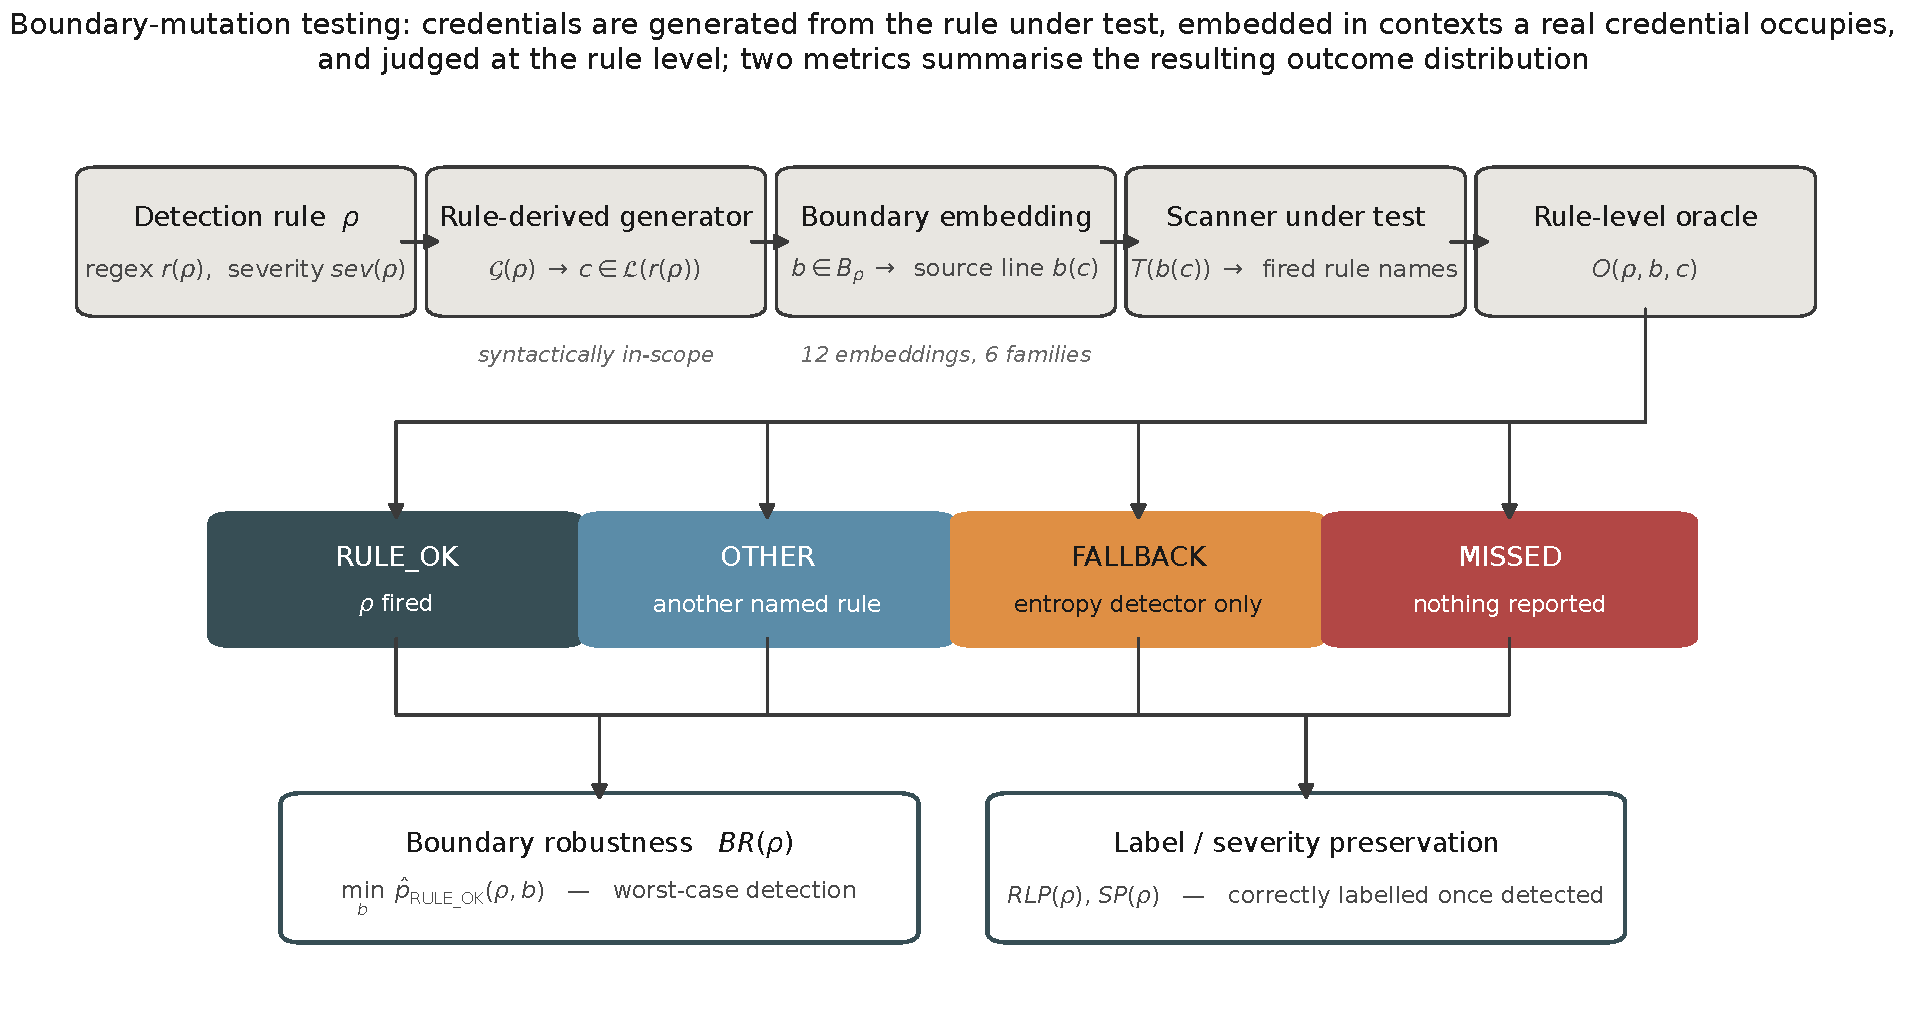
\includegraphics[width=\columnwidth]{fig00_framework.pdf}
\caption{Boundary-mutation testing. A credential generated from the rule under test is embedded in a context that real credentials occupy, and the outcome is classified at the rule level.}
\label{fig:framework}
\end{figure}

\section{Research Questions}
\label{sec:rqs}

\noindent\RQ{1} \emph{Does rule-level detection depend on the context surrounding a credential?}

\noindent\RQ{2} \emph{What mechanism produces the dependence, and how likely is it to affect a credential?}

\noindent\RQ{3} \emph{Across six scanners and their full rule tables, which boundary defects occur, and do they travel with reused rules?}

\noindent\RQ{4} \emph{How do the scanners compare in coverage once generator bias, rule lineage and duplicated providers are controlled?}

\noindent\RQ{5} \emph{Can the defects be repaired without losing detections or adding false positives, in the versions practitioners run today?}

\noindent\RQ{6} \emph{How do the scanners handle escaped, interpolated, marked-up and transformed credentials, and how exposed is real code to the boundary defects?}

\section{Related Work}
\label{sec:related}

\textbf{Secret detection.} Meli et al.~\cite{meli2019} measured leakage on GitHub at scale. Later work addresses false positives~\cite{saha2020,rahman2019} and tool accuracy~\cite{basak2022}. Basak et al.\ compare nine detection tools on a curated benchmark~\cite{basak2023comparative} and contribute the benchmark, SecretBench~\cite{basak2023secretbench}; Li et al.\ evaluate detection for Android applications~\cite{li2025android}. These studies compare tools on credentials collected from the field, so the credential and its surroundings vary together and the tool is the treatment. We hold the credential's language fixed---it is generated from the rule---and make the \emph{context} the treatment, so a change in outcome is attributable to the boundary. We have not found a prior study that varies the context systematically while attributing outcomes at the rule level, nor prior reports of the defects in Section~\ref{sec:rq3}.

\textbf{Mutation and metamorphic testing.} Classical mutation testing perturbs the program to assess a test suite~\cite{jia2011,demillo1978}; we perturb the input of a rule table. The context mutations are metamorphic relations~\cite{chen2018metamorphic,segura2016}: re-quoting a credential or moving it into a YAML file does not change whether it is a credential. Generating inputs from a formal description relates to grammar-based fuzzing~\cite{godefroid2008} and property-based testing~\cite{claessen2000}; here the description is the detector's own expression, so a generated value is in scope for the rule by construction. Studies of regular-expression use~\cite{chapman2016,michael2019} document that developers misjudge anchoring and class semantics; both defect classes below are instances.

\textbf{Benchmark design as a confound.} Benchmark construction, not only technique quality, drives measured outcomes~\cite{liem2020,herbold2020}. Section~\ref{sec:rq4} treats the generator of a corpus, the lineage of rule tables and the duplication of providers as variables to control.

\section{Boundary-Mutation Testing}
\label{sec:method}

\subsection{Definition}

Let $\rho$ be a detection rule with expression $r(\rho)$ and severity $sev(\rho)$, and $\mathcal{G}(\rho)$ a generator of strings in $\mathcal{L}(r(\rho))$. Let $B$ be a set of \emph{embeddings}, each $b\in B$ mapping a credential $c$ to a line of source $b(c)$ in which $c$ appears as a real credential would, and let $T(b(c))$ be the set of rules tool $T$ fires.

\textbf{Syntactic, not semantic, validity.} Write $C_\rho\subseteq\mathcal{L}(r(\rho))$ for the strings the provider would actually issue. The generator guarantees membership in $\mathcal{L}(r(\rho))$ only. A miss is therefore an internal inconsistency in the rule: its author declared, by writing $r(\rho)$, that such strings are to be reported in such contexts, and they were not. It is not a claim that the particular string would be issued; Section~\ref{sec:rq2} computes marginal probabilities under an explicit issuance model for that reason.

\textbf{The metamorphic relation.} For a credential $c$ and embeddings $b_i,b_j$ both applicable to $\rho$,
\[
\mathit{MR}(c,b_i,b_j):\quad \rho\in T(b_i(c)) \;\Longleftrightarrow\; \rho\in T(b_j(c)).
\]
The relation asserts preservation of detectability under a semantics-preserving change of context, and localises a defect without a ground-truth detector. An embedding is \emph{applicable} when it keeps the credential in $\mathcal{L}(r(\rho))$; forcing a final character the rule's class excludes would make a miss correct. Each outcome is one of \textsc{rule\_ok} ($\rho$ fired), \textsc{other} (another named rule fired), \textsc{fallback} (only an unanchored fallback detector fired) or \textsc{missed}.

\subsection{Metrics}
\label{sec:metrics}

With $\hat p_{\textsc{x}}(\rho,b)$ the rate of outcome \textsc{x} and $B_\rho$ the applicable embeddings, \emph{boundary robustness} is the worst case over contexts,
\begin{equation}
BR(\rho)=\min_{b\in B_\rho}\hat p_{\textsc{rule\_ok}}(\rho,b);
\end{equation}
\emph{rule-label preservation} is the share of detected credentials reported under their own rule,
\begin{equation}
RLP(\rho)=\frac{\sum_{b}\hat p_{\textsc{rule\_ok}}(\rho,b)}{\sum_{b}\bigl(1-\hat p_{\textsc{missed}}(\rho,b)\bigr)};
\end{equation}
and \emph{severity preservation} $SP(\rho)$ is the same ratio with the numerator counting findings reported at $sev(\rho)$. $RLP<1$ means findings are attributed to the wrong rule, $SP<1$ that they are reported at the wrong severity. $SP$ needs a severity oracle, which only the primary subject provides; the external tools are measured by $BR$ and $RLP$ and by the total-failure counts of Section~\ref{sec:rq3}.

\subsection{The battery}
\label{sec:battery}

Table~\ref{tab:battery} lists the embeddings. Each family is a distinct mechanism by which a character comes to sit next to a credential, which is all an anchoring construct can observe; the battery is representative of mechanisms, not exhaustive. Two extension contexts---a credential followed by \texttt{\&} in a query string, and minimal-pair controls with one space before the terminator---are reported but kept out of $BR$. Seventeen further contexts in five families (escaping, interpolation, markup, file syntax, transformed values) are reported in Section~\ref{sec:rq6}.

\begin{table}[t]
\centering
\caption{The boundary battery}
\label{tab:battery}
\footnotesize
\setlength{\tabcolsep}{3pt}
\begin{tabular}{@{}p{1.55cm}p{2.85cm}p{3.35cm}@{}}
\toprule
Family & Embedding & Mechanism exercised \\
\midrule
Assignment & quoted, single-quoted, unquoted & canonical shape; quote; no delimiter \\
Structured data & YAML, JSON, \texttt{.env} & configuration syntax \\
Expression & call argument \texttt{f(v)} & credential passed programmatically \\
Collection & list member / keyword argument & separator after the value \\
URL & query parameter & where credentials often leak \\
Lexical & extra whitespace & whitespace as terminator \\
Final character & ends in \texttt{\_}, ends in \texttt{-} & word and non-word terminal \\
\bottomrule
\end{tabular}
\end{table}

\textbf{A control that proved necessary.} An early harness used the identifier \texttt{SECRET} and measured 100\% detection everywhere: the identifier triggered the subject's generic keyword rules, which masked the failure of the rule under test. All embeddings use neutral identifiers. A tool-level oracle could not have told the two situations apart.

\section{Study Design}
\label{sec:design}

\subsection{Scanners}
\label{sec:subjects}

Table~\ref{tab:tools} lists the six scanners. The primary subject is the secret scanner of GitHub Autopilot at commit \texttt{38b2013}: 43 rules with per-rule severities and an entropy fallback. The others are official releases, pinned by version and verified by SHA-256 (the digests are in the replication package).

\begin{table}[t]
\centering
\caption{Scanners studied. ``Types'' counts the credential types generated from each rule table and included in the battery.}
\label{tab:tools}
\footnotesize
\setlength{\tabcolsep}{3pt}
\begin{tabular}{@{}llrl@{}}
\toprule
Scanner & Version & Types & Rule source \\
\midrule
Primary subject (AP) & \texttt{38b2013} & 24 & own (Python) \\
Gitleaks (GL) & 8.21.2 & 183 & own (Go, TOML table) \\
TruffleHog (TH) & 3.82.13 & 566 & own (Go detectors) \\
Nosey Parker (NP) & 0.24.0 & 109 & own (Rust, YAML) \\
Kingfisher (KF) & 2.11.1 & 356 & 461 of 488 from Betterleaks \\
detect-secrets (DS) & 1.5.0 & --- & 27 plugins; no rule table \\
\midrule
Total & & 1{,}238 & \\
\bottomrule
\end{tabular}
\end{table}

\subsection{Five generators}
\label{sec:generators}

A corpus generated from one tool's rules favours that tool, since every type in it is a shape the tool declares. Credential types are therefore drawn from five rule tables. From Gitleaks, each rule's secret group (the generic catch-all rule, which names no provider, is not a generator). From TruffleHog, each detector whose matching uses exactly one expression: of its detectors, 213 need two or more patterns, 9 build theirs in a helper and 7 have none, and they are excluded and counted. From Nosey Parker, the rules of its default ruleset---162 of 183; its opt-in rulesets for identifiers such as AWS key IDs and for password hashes are not claims it makes by default, and a first run that included them found, as it should, that it covered none of them. From Kingfisher, every rule that reports on its own and is not restricted to file paths (41 depend on another rule's match, 47 are hidden components and 8 are path rules). detect-secrets declares its formats in plugin code, not in a table of expressions, so it is a scanner here and not a generator; since a corpus can favour only a tool whose rules generated it, a tool that generates none is never favoured.

Go and Rust regular-expression syntax is translated before generation (ASCII classes, POSIX classes, Rust's verbose mode, which ignores whitespace inside classes too). A sample is kept only if it passes the generating tool's own filters: Gitleaks' keyword prefilter, entropy threshold and allowlists; TruffleHog's keywords; for Nosey Parker and Kingfisher, the rule's whole translated pattern must find the value in the canonical line. A translation error therefore shows up as a tool not covering its own type, which is measured: AP, GL and NP cover all of their own types, KF 354 of 356, TH 533 of 566. Types with fewer than $n=20$ valid samples in 300 draws are excluded (87, listed).

\subsection{Oracle: frozen expected rule and label matching}
\label{sec:oracle}

For each tool and type the expected rule is the rule the tool fires most often in the canonical context; the type is \emph{covered} when that rule fires on at least half the canonical samples, and the rule is then frozen for every other context. Ties are broken towards a rule naming the type's own provider, then by name, so the choice does not depend on set iteration order. A covered type counts as \emph{label-matched} only when the frozen rule names the type's own provider (equal names, one a prefix of the other, or a shared prefix of five characters). Boundary and encoding results use label-matched types only; detections under another provider's label are reported as mislabelling.

\subsection{Comparison design}
\label{sec:comparedesign}

\textbf{Lineage-neutral types.} Each pair of tools is compared only on types generated by tables outside both tools' lineages. Kingfisher's imported rules share Gitleaks' identifiers and expressions, so Gitleaks and Kingfisher form one lineage: neither's types are neutral ground for a comparison involving the other.

\textbf{Providers as the unit.} Several tables declare the same provider's credential---GitHub's \texttt{ghp\_} token is a Gitleaks, a TruffleHog, a Nosey Parker and a Kingfisher type---so types are not independent. The 1{,}238 types belong to 760 providers, up to 34 types each. Every comparison is reported twice: an exact sign test on discordant types, and an exact sign test on providers, scoring each provider by the share of its types one tool covers minus the share the other covers. Differences in coverage carry 95\% percentile intervals from a bootstrap that resamples providers ($10^4$ replicates, seeded). $p$-values are Holm-adjusted over the 15 pairs. Two sensitivity analyses repeat the comparison with one type per provider and with coverage requiring 80\% of canonical samples.

\subsection{Scanner settings that would bias the oracle}
\label{sec:settings}

Three defaults would have measured something other than the rules. Nosey Parker's report prints at most three matches per finding and three file provenances per match: on a 2{,}000-file probe it reported 300 of the 2{,}000 files. Kingfisher deduplicates identical secrets across files, so a value detected in one context hides the same value in every other. detect-secrets checks candidate secrets against the providers' APIs over the network by default; our first run attempted connections to Slack, Stripe and Telegram, which the sandbox's network policy refused. All three are switched off (no match limits; \texttt{--no-dedup}; \texttt{--no-verify}), as is TruffleHog's live verification; Gitleaks and Nosey Parker do not verify. TruffleHog is not deterministic on identical input, so it is run three times and only detections present in every run are kept; in the final battery none was unstable.

\subsection{Determinism and verification}
\label{sec:determinism}

All harnesses are seeded (\texttt{20260823}). The six-scanner battery gives byte-identical output, wall time aside, under two values of \texttt{PYTHONHASHSEED}. A verification script re-derives every number in this paper from the raw output, and a continuous-integration workflow runs it, the harness regression tests, and a from-scratch replication of the seeded Gitleaks full-table battery on every change to the package.

\section{RQ1 and RQ2: The Primary Subject}
\label{sec:rq1}
\label{sec:rq2}

On the primary subject's 24 analysable rules ($n=120$ per cell) rule-level detection never falls below $0.9976$ in ten of twelve contexts and is $1.0000$ for a final underscore. A final hyphen, which the affected rules' own classes permit, drops it to $\mathbf{0.5233}$: $23.2\%$ of samples are rescued only by the entropy fallback and $24.5\%$ are reported by nothing (Fig.~\ref{fig:heatmap}). Five rules are fragile (Table~\ref{tab:metrics}).

\begin{figure}[t]
\centering
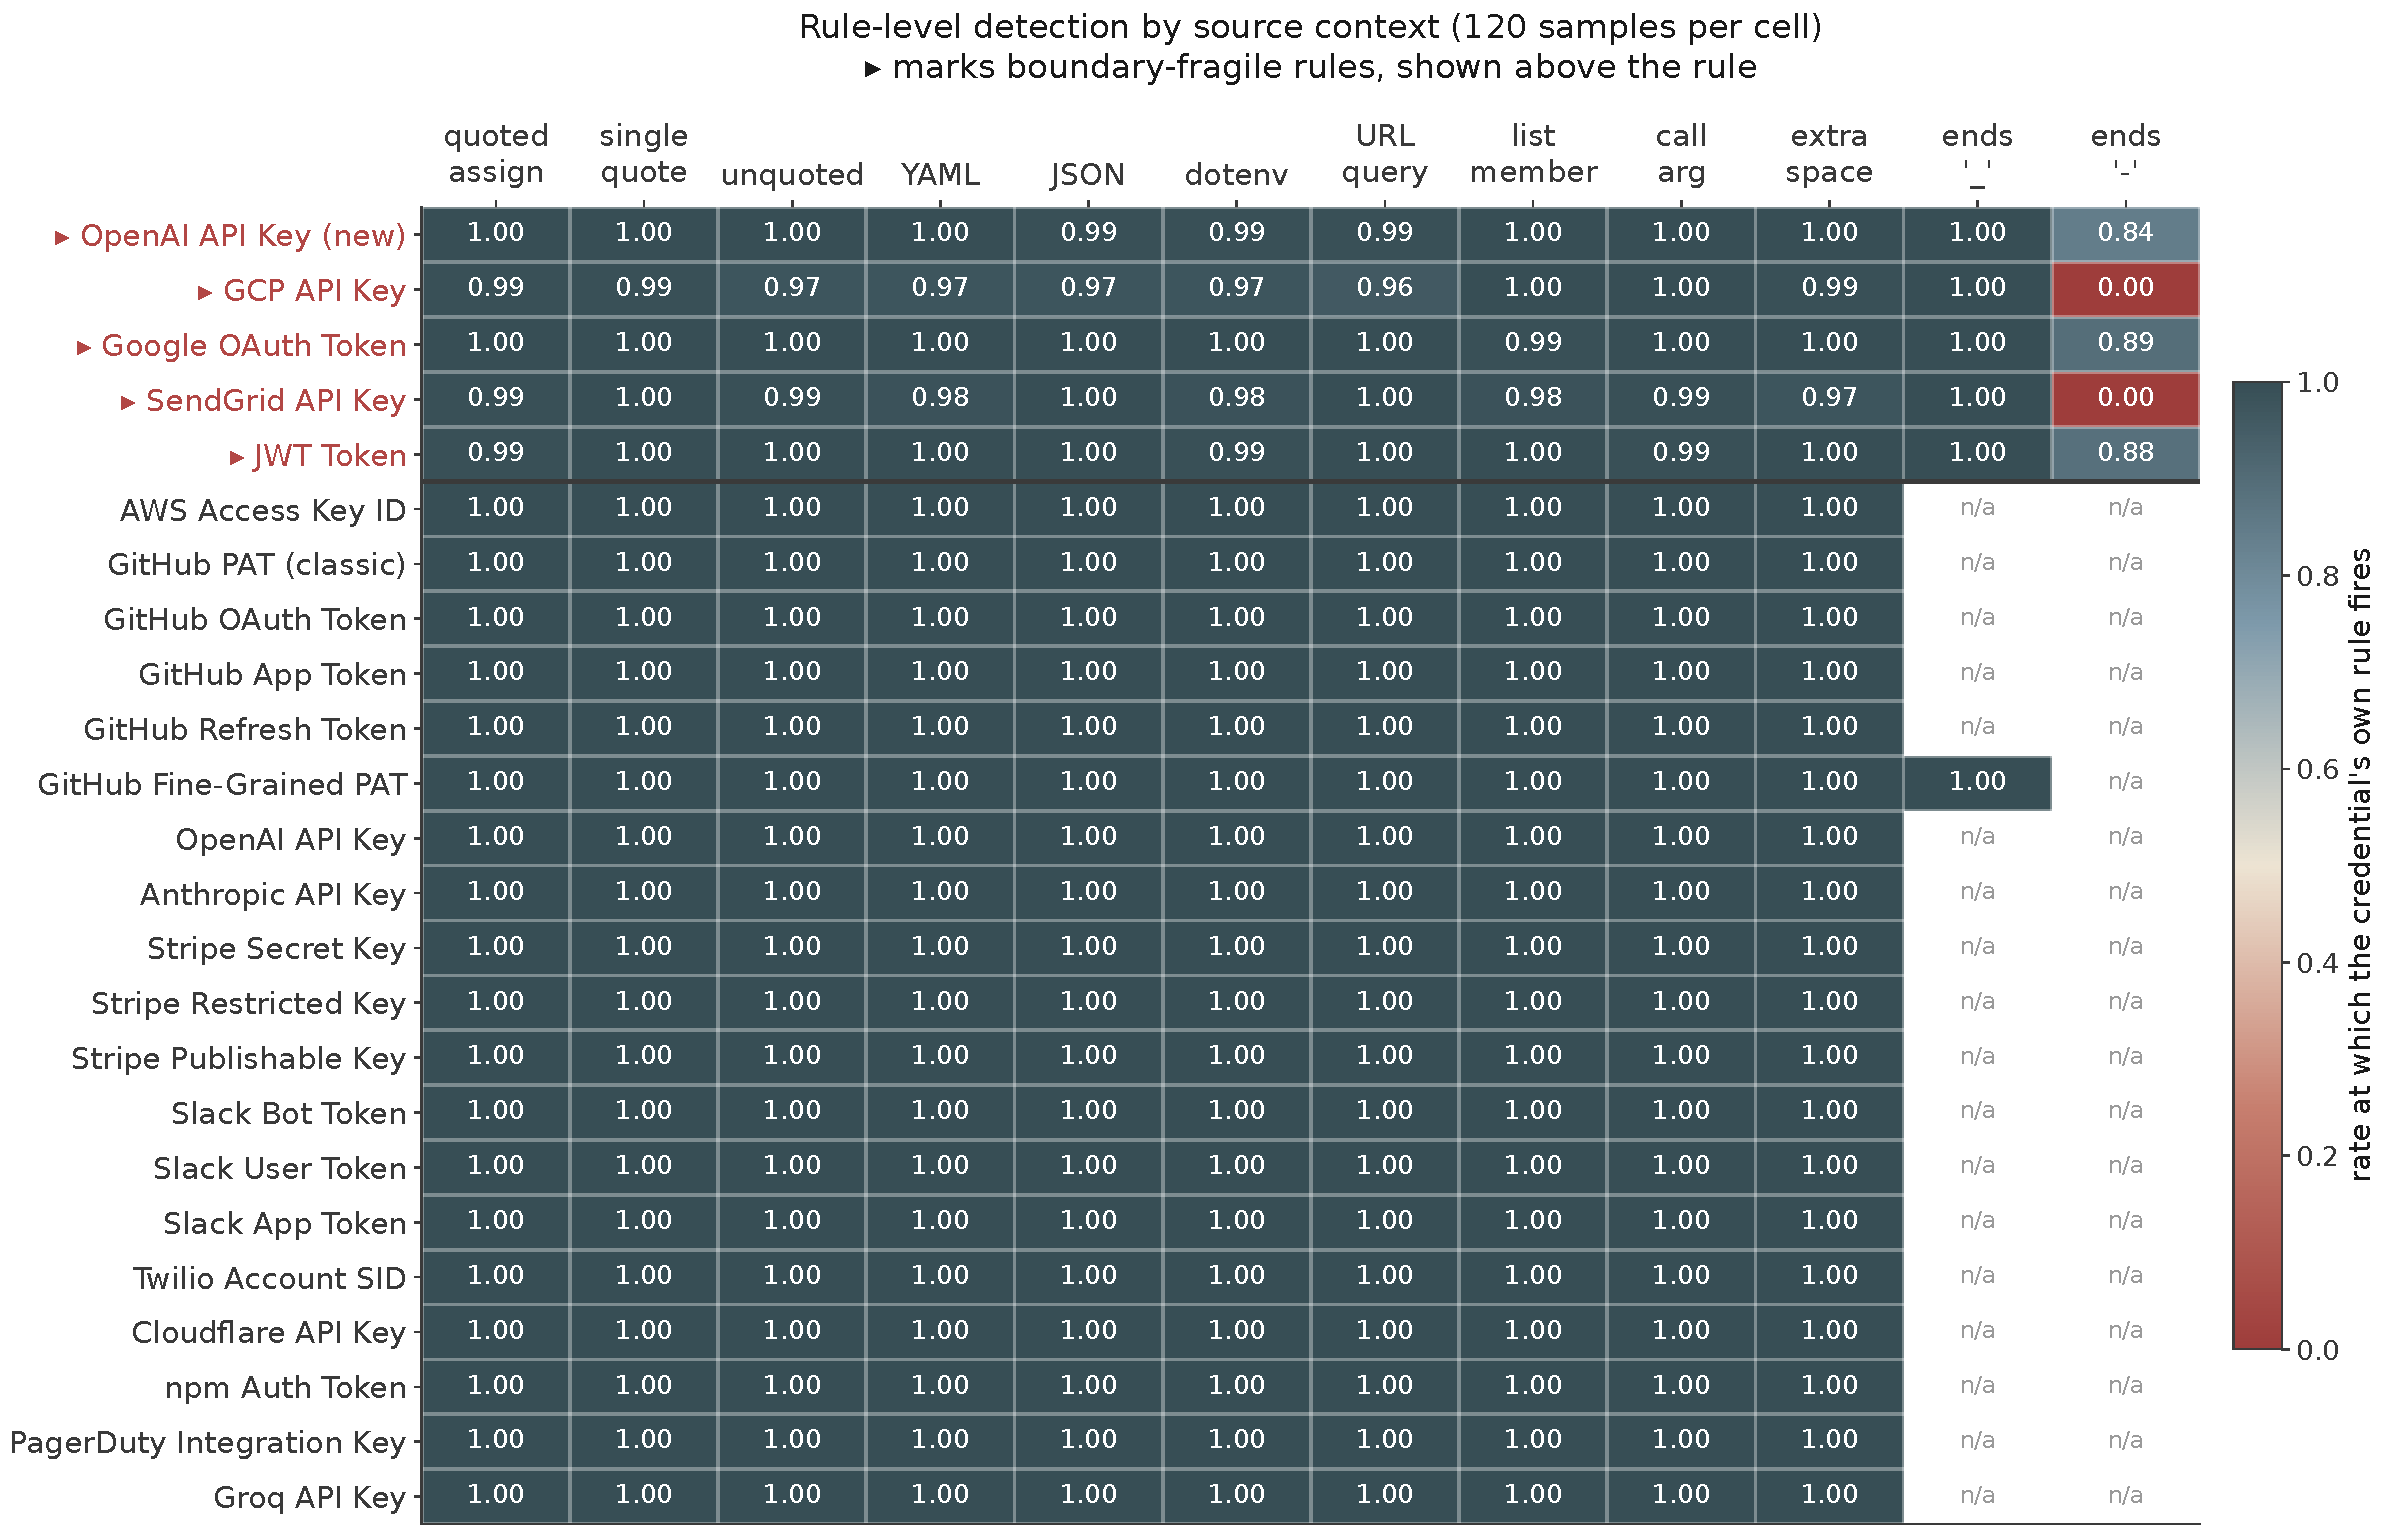
\includegraphics[width=\columnwidth]{fig02_mutation_heatmap.pdf}
\caption{Primary subject: rule-level detection across 24 rules and 12 contexts ($n=120$ per cell).}
\label{fig:heatmap}
\end{figure}

\begin{table}[t]
\centering
\caption{Primary subject: the five rules below $1.0000$ on any metric}
\label{tab:metrics}
\footnotesize
\begin{tabular}{@{}llrrr@{}}
\toprule
Rule & Severity & $BR$ & $RLP$ & $SP$ \\
\midrule
SendGrid API Key & \textsc{critical} & 0.0000 & 1.0000 & 1.0000 \\
GCP API Key & \textsc{high} & 0.0000 & 0.9116 & 0.9116 \\
OpenAI API Key (new) & \textsc{critical} & 0.8417 & 0.9861 & 0.9861 \\
JWT Token & \textsc{high} & 0.8833 & 1.0000 & 1.0000 \\
Google OAuth Token & \textsc{high} & 0.8917 & 1.0000 & 1.0000 \\
\bottomrule
\end{tabular}
\end{table}

\textbf{Mechanism.} Each fragile rule ends with \verb|\b| right after a class that contains a hyphen, e.g.\ \lstinline!\bSG\.[a-zA-Z0-9_-]{22}\.[a-zA-Z0-9_-]{43}\b!. A hyphen is not a word character, so when the credential ends in one and a quote follows, no word boundary exists and the match fails---before any suppression logic runs. Fixed-count quantifiers (\texttt{\{43\}}, \texttt{\{35\}}) leave no room to backtrack and fail totally; variable-count ones (\texttt{\{50,\}}, \texttt{\{10,\}}, \texttt{\{68,\}}) backtrack and report a credential one character short. The entropy fallback's class excludes the dot, so dotted credentials (SendGrid, Google OAuth, JWT) are missed silently, while dotless ones (GCP, OpenAI) are rescued and downgraded to \textsc{medium}: $BR$ and $RLP$ separate the two failure modes, which a tool-level metric would score as detected.

\textbf{Marginal probability.} The rates are conditional on a final hyphen. For a tail drawn uniformly from a 64-symbol alphabet, $P(\text{final ``-''})=1/64$: one SendGrid key in 64 is missed outright and one GCP key in 64 is downgraded. For JWTs the last character carries only the residual bits of a base64url-encoded signature; ``-'' (index 62) is reachable only when the signature length is $0\bmod 3$, so an HS256 token (32 bytes) is structurally immune and an HS384 token (48 bytes) is not (1 in 548).

\textbf{Repair.} Replacing the trailing \verb|\b| with \verb+(?![A-Za-z0-9_])+ restores $BR=1.0$ on all five rules and adds no finding on 292{,}527 lines of real code (67 findings before and after). A first candidate, \verb+(?=[^\w-]|$)+, repairs the defect too, but regresses SendGrid and GCP to total failure on a case the original handled: a credential ending in a letter and followed by a hyphen. We found that only by running an oracle-based probe against the fix. It is the design principle of Section~\ref{sec:rq5}: a repair must accept everything the original accepts.

\section{RQ3: Boundary Defects Across Six Scanners}
\label{sec:rq3}

Table~\ref{tab:prevalence} gives, for each scanner and context, how many of its label-matched types the context defeats entirely, with a provider-cluster bootstrap interval for the share. Two defect classes account for every large count.

\begin{table*}[t]
\centering
\caption{Label-matched types defeated entirely (no sample detected) by each context, with the share's 95\% provider-cluster bootstrap interval. The trailing-hyphen row counts only types whose format allows a final hyphen. AP's eight in every unquoted context are its Cloudflare and Heroku rules, which require a quoted value.}
\label{tab:prevalence}
\footnotesize
\setlength{\tabcolsep}{4pt}
\begin{tabular}{@{}lrrrrrr@{}}
\toprule
Context & AP & Gitleaks & TruffleHog & Nosey Parker & Kingfisher & detect-secrets \\
\midrule
label-matched types & 67 & 427 & 688 & 203 & 616 & 82 \\
\midrule
unquoted / YAML / \texttt{.env} & 8 / 8 / 8 & 5 / 5 / 5 & 0 / 0 / 2 & 1 / 3 / 1 & 0 / 0 / 0 & 0 / 0 / 0 \\
call argument, `\texttt{)}' & 8 & \textbf{302} [0.56, 0.86] & 3 & 1 & \textbf{436} [0.60, 0.81] & 0 \\
query string, `\texttt{\&}' & 8 & \textbf{305} [0.56, 0.87] & 3 & 1 & \textbf{436} [0.60, 0.82] & 0 \\
keyword argument, `\texttt{,}' & 8 & 198 [0.35, 0.59] & 3 & 1 & 268 [0.35, 0.53] & 0 \\
\midrule
trailing hyphen & 6 / 12 & 3 / 119 & \textbf{97 / 132} [0.64, 0.82] & 7 / 43 & 2 / 173 & 0 / 30 \\
\bottomrule
\end{tabular}
\end{table*}

\subsection{An explicit terminator allowlist: Gitleaks}
\label{sec:rq3-gitleaks}

Most Gitleaks rules end with the group \lstinline!(?:['|\"|\n|\r|\s|\x60|;]|$)!: a character class, written as if it were an alternation, admitting a quote, `\texttt{|}', whitespace, a backtick, `\texttt{;}' or the end of input after the secret, and nothing else. A credential followed by `\texttt{)}', `\texttt{,}', `\texttt{\&}', `\texttt{]}', `\texttt{\}}' or a backslash is not reported. A full-table harness runs the battery over every Gitleaks rule with $n=40$, generating from each rule's own secret group, so the expected rule is the generating one. Of 195 rules, 183 are analysed and 135 lose more than half their values in some context: 134 of them in the call-argument context, 95 of those also after a comma; the remaining one, a Hugging Face rule, loses values followed by a newline, because its pattern ends in \verb|$| without \texttt{(?m)}. Of the 134, 133 carry the terminator group; the other, the Hugging Face access-token rule, lacks `\texttt{(}' in its \emph{leading} class. Of the 50 prefix rules without the group, 49 pass (Fisher exact test, $p=3.3\times10^{-24}$; the association was predicted from the configuration, so the test adds prevalence, not mechanism). At 1{,}238 types the defect reaches 302 of Gitleaks' 427 label-matched types (Table~\ref{tab:prevalence}).

\subsection{Inheritance: Kingfisher}
\label{sec:rq3-inherit}

Kingfisher's built-in table is generated from Betterleaks' (461 rules) and Google's Veles detectors~\cite{osvscalibr} (26), with one rule of its own. Betterleaks is maintained by Gitleaks' original author, and its table keeps Gitleaks' rule identifiers and expression forms, including a revised terminator, \lstinline!(?:\\?['"\x60]|[\s;]|\\[nr]|$)!. The revision accepts an escaped quote and a line break, but still no `\texttt{)}', `\texttt{,}' or `\texttt{\&}'. Kingfisher is a separate implementation in another language, on a different regular-expression engine; the defect is not in its code, and it is present at the same scale: a trailing `\texttt{)}' defeats 436 of its 616 label-matched types, against 302 of 427 for Gitleaks, with overlapping intervals. A boundary assumption written into a rule table travels with the table.

\subsection{An implicit word-boundary anchor: TruffleHog}
\label{sec:rq3-trufflehog}

TruffleHog is robust to every terminator in the battery (at most 3 of 688 types), but a trailing hyphen defeats 97 of the 132 label-matched types whose formats allow one. The mechanism is the primary subject's: 381 detector patterns in 3.82.13 end in \verb|\b| after a class containing a non-word character, e.g.\ \lstinline!\b(r8_[0-9A-Za-z-_]{37})\b!. A valid Replicate token ending in `\texttt{-}' is missed when quoted or at the end of a line, while an \emph{invalid} 41-character string \texttt{r8\_\ldots-x} is reported, truncated to 40. Estimating $P(\text{final ``-''})$ from 1{,}000 draws of each type's own generator, 91 of the 132 types have a marginal failure probability of at least 1 in 100 (maximum 0.061).

\subsection{Scanners without either defect}

On Nosey Parker, 7 of 43 applicable types fail on a trailing hyphen and at most 3 of 203 in any other boundary context; some of its patterns end in an explicit negated class over the secret's alphabet, such as \lstinline!(?:[^a-z0-9-]|$)!. detect-secrets fails none of its 82 label-matched types in any boundary context. Neither defect, then, is a necessary cost of pattern-based detection.

\section{RQ4: Comparison}
\label{sec:rq4}

\textbf{Generator bias.} Table~\ref{tab:coverage} counts label-matched types covered, by generator. Each tool covers nearly every type its own table generated, and the shared lineage shows: Kingfisher covers 167 of Gitleaks' 183 types, and Gitleaks 174 of Kingfisher's 356, against at most 47 of any other table's. A pooled comparison is therefore weighted towards whichever tables contributed most types.

\begin{table}[t]
\centering
\caption{Label-matched types covered, by the table that generated them}
\label{tab:coverage}
\footnotesize
\setlength{\tabcolsep}{3pt}
\begin{tabular}{@{}lrrrrrr@{}}
\toprule
Covered by $\downarrow$ / from $\rightarrow$ & AP & GL & TH & NP & KF & All \\
 & 24 & 183 & 566 & 109 & 356 & 1{,}238 \\
\midrule
AP & 24 & 10 & 6 & 13 & 14 & 67 \\
Gitleaks & 13 & 183 & 23 & 34 & 174 & 427 \\
TruffleHog & 11 & 36 & 533 & 33 & 75 & 688 \\
Nosey Parker & 11 & 33 & 7 & 109 & 43 & 203 \\
Kingfisher & 12 & 167 & 47 & 36 & 354 & 616 \\
detect-secrets & 12 & 22 & 5 & 15 & 28 & 82 \\
\bottomrule
\end{tabular}
\end{table}

\textbf{Lineage-neutral, provider-clustered comparison.} Table~\ref{tab:neutral} reports every pair. The primary subject covers fewer types than Gitleaks, TruffleHog, Nosey Parker and Kingfisher, with types or providers as the unit, after Holm adjustment, with one type per provider, and at the 80\% coverage threshold. Its comparison with detect-secrets illustrates why the clustering matters: by type the difference is significant ($p_{\text{Holm}}=0.015$), by provider it is 10 to 10 ($p=1$), and the coverage interval includes zero. We report no difference. Nor is there one between Gitleaks and TruffleHog or between TruffleHog and Kingfisher, under any analysis.

\begin{table*}[t]
\centering
\caption{Lineage-neutral comparison. ``Types'': label-matched types covered by only the first / only the second tool, on types generated outside both tools' lineages. ``Providers'': providers on which the first / the second tool covers the larger share. $p$: exact sign test, Holm-adjusted over 15 pairs. $\Delta$: difference in coverage (first minus second), with 95\% provider-cluster bootstrap interval.}
\label{tab:neutral}
\footnotesize
\setlength{\tabcolsep}{4pt}
\begin{tabular}{@{}llrrrrrr@{}}
\toprule
Pair & Generators & $n$ & Types & $p$ & Providers & $p$ & $\Delta$ [95\% CI] \\
\midrule
AP vs Gitleaks & NP, TH & 675 & 3 / 41 & $1.6\times10^{-8}$ & 2 / 30 & $2.5\times10^{-6}$ & $-0.056$ [$-0.083$, $-0.032$] \\
AP vs TruffleHog & GL, KF, NP & 648 & 7 / 114 & $7.6\times10^{-25}$ & 4 / 62 & $3.1\times10^{-13}$ & $-0.165$ [$-0.218$, $-0.118$] \\
AP vs Nosey Parker & GL, KF, TH & 1{,}105 & 10 / 63 & $1.9\times10^{-9}$ & 4 / 29 & $8.7\times10^{-5}$ & $-0.048$ [$-0.075$, $-0.022$] \\
AP vs Kingfisher & NP, TH & 675 & 2 / 66 & $2.2\times10^{-16}$ & 2 / 54 & $6.2\times10^{-13}$ & $-0.095$ [$-0.124$, $-0.067$] \\
AP vs detect-secrets & GL, KF, NP, TH & 1{,}214 & 26 / 53 & 0.015 & 10 / 10 & 1 & $-0.022$ [$-0.074$, $0.018$] \\
Gitleaks vs TruffleHog & AP, NP & 133 & 19 / 16 & 1 & 12 / 10 & 1 & $0.023$ [$-0.117$, $0.146$] \\
Gitleaks vs Nosey Parker & AP, TH & 590 & 26 / 8 & 0.015 & 24 / 7 & 0.013 & $0.030$ [$0.009$, $0.052$] \\
Gitleaks vs Kingfisher & AP, NP, TH & 699 & 5 / 30 & $1.6\times10^{-4}$ & 5 / 29 & $2.7\times10^{-4}$ & $-0.036$ [$-0.053$, $-0.019$] \\
Gitleaks vs detect-secrets & AP, NP, TH & 699 & 46 / 8 & $1.1\times10^{-6}$ & 33 / 4 & $9.8\times10^{-6}$ & $0.054$ [$0.031$, $0.081$] \\
TruffleHog vs Nosey Parker & AP, GL, KF & 563 & 74 / 39 & 0.0077 & 51 / 17 & $2.7\times10^{-4}$ & $0.062$ [$0.004$, $0.119$] \\
TruffleHog vs Kingfisher & AP, NP & 133 & 13 / 17 & 1 & 7 / 10 & 1 & $-0.030$ [$-0.154$, $0.105$] \\
TruffleHog vs detect-secrets & AP, GL, KF, NP & 672 & 118 / 40 & $4.4\times10^{-9}$ & 66 / 8 & $2.2\times10^{-11}$ & $0.116$ [$0.017$, $0.209$] \\
Nosey Parker vs Kingfisher & AP, TH & 590 & 6 / 47 & $5.2\times10^{-8}$ & 6 / 45 & $2.0\times10^{-7}$ & $-0.070$ [$-0.095$, $-0.046$] \\
Nosey Parker vs detect-secrets & AP, GL, KF, TH & 1{,}129 & 70 / 43 & 0.042 & 32 / 9 & 0.0022 & $0.024$ [$-0.024$, $0.068$] \\
Kingfisher vs detect-secrets & AP, NP, TH & 699 & 72 / 9 & $3.2\times10^{-12}$ & 58 / 5 & $2.2\times10^{-11}$ & $0.090$ [$0.063$, $0.119$] \\
\bottomrule
\end{tabular}
\end{table*}

The coverage differences are small in absolute terms---at most 17 percentage points---because most generated types are covered by few tools: a neutral type set is dominated by formats only its own lineage declares. Coverage is one dimension of quality; Section~\ref{sec:rq6} measures false positives.

\textbf{Mislabelling.} Without label matching the primary subject would be credited with 122 types it detects under another provider's label, 98 of them under a PagerDuty rule that at the measured commit is \verb|\b[a-z0-9]{32}\b|---any 32-character lowercase word. The other tools mislabel 4 to 8 types each. A tool-level oracle would have counted every one as a detection.

\textbf{Ten types cannot rank.} The first version of this study compared three tools on ten shared types and found no significant difference: per-type detection is nearly deterministic, so the type is the unit and even a perfect 4/0 split has $p=0.125$. That null result was correct for ten types. The raw ten-type numbers, which favoured the primary subject, pointed the wrong way: those corpora were built from published prefix-and-length specifications, the shallow shape the subject's rules encode.

\section{RQ5: Repairs, Validated, in Current Releases}
\label{sec:rq5}

A repair to a boundary construct can fail in the direction the battery does not probe: it can become \emph{stricter} than the construct it replaces (Section~\ref{sec:rq2}). Every repair below therefore only widens the set of strings a rule accepts, so it cannot lose a match position the original accepts; and each is checked twice, on the battery that found the defect and on the 31-project corpus of Section~\ref{sec:rq6} (38{,}309 files, 9{,}870{,}820 lines in nine languages) for findings it adds \emph{and} removes. Added findings are inspected by hand.

\subsection{Gitleaks}

Three repairs of the terminator group were evaluated on Gitleaks 8.21.2 (Table~\ref{tab:glrepair}). \emph{R1} adds the missing source-code delimiters---\texttt{,} \texttt{)} \texttt{]} \texttt{\}} \texttt{>} \texttt{<} \texttt{\&} and backslash---to the class, and the line break to the two Hugging Face rules (the access-token rule's leading class also gains the `\texttt{(}' its sibling already has). \emph{R2} replaces the class with the complement of the secret's own alphabet, keeping every character the original accepts. \emph{R1P} is R1 on every rule except \texttt{generic-api-key}, the catch-all.

\begin{table}[t]
\centering
\caption{Gitleaks 8.21.2: rules losing more than half their values in some context (of 183), and findings changed on 9.87M lines of real code (1{,}101 before)}
\label{tab:glrepair}
\footnotesize
\begin{tabular}{@{}lrrr@{}}
\toprule
Table & Fragile rules & Added & Removed \\
\midrule
original & 135 & --- & --- \\
R1 & 0 & 25 & 0 \\
R2 & 0 & 53 & 0 \\
R1P & 1 (the catch-all) & \textbf{0} & \textbf{0} \\
\bottomrule
\end{tabular}
\end{table}

Every finding R1 and R2 add comes from \texttt{generic-api-key}, and none is a live credential: test fixtures, registry mocks, an environment-variable reference, an identifier, a URL form key and base64 of a fixture string (R1 adds 19 of its 25 before a backslash). R2 also truncates values whose real alphabet is wider than the catch-all's, reporting \texttt{whsec\_\ldots} up to its first `\texttt{+}'. For the provider rules both repairs add nothing. R1P is the repair we recommend: every provider rule repaired, no change in findings on real code. That last result shows absence of cost, not presence of benefit: the corpus contains no provider credential in a context the repair newly accepts.

\subsection{The current releases}
\label{sec:current}

Gitleaks 8.30.1, the latest release at the time of writing~\cite{gitleaks830}, rewrote the group as a proper class, \lstinline!(?:[\x60'"\s;]|\\[nr]|$)!, and in doing so fixed the Hugging Face newline case; 151 of its 222 rules end in it, and it still rejects `\texttt{)}', `\texttt{,}' and `\texttt{\&}'. Table~\ref{tab:current} runs minimal reproducers, with seeded random values (sequential placeholders are discarded by these tools' filters and would test the filter instead), against every current release. The same delimiter addition, applied to 8.30.1 (150 rules) and to Betterleaks 1.9.0 (335 rules), fixes every boundary case and changes no finding on the real-code corpus: 1{,}057 findings before and after for Gitleaks 8.30.1, 1{,}358 for Betterleaks, none added, none removed. A credential inside an escaped JSON string is missed by every tool with or without the repair: there the backslash is rejected between the keyword and the value, a separate leading-side defect that we do not repair.

\begin{table}[t]
\centering
\caption{Minimal reproducers on the releases current at the time of writing (GL Gitleaks, BL Betterleaks, KF Kingfisher, TH TruffleHog). F: found; \textbf{M}: missed; +R: with the repair.}
\label{tab:current}
\footnotesize
\setlength{\tabcolsep}{2.2pt}
\begin{tabular}{@{}lccccccc@{}}
\toprule
 & \multicolumn{2}{c}{GL 8.30.1} & \multicolumn{2}{c}{BL 1.9.0} & KF 2.14.0 & \multicolumn{2}{c}{TH 3.99.3} \\
Case & & +R & & +R & & & +R \\
\midrule
key in quotes & F & F & F & F & F & & \\
key, `\texttt{)}' & \textbf{M} & F & \textbf{M} & F & \textbf{M} & & \\
key, `\texttt{\&}' & \textbf{M} & F & \textbf{M} & F & \textbf{M} & & \\
key, `\texttt{,}' & \textbf{M} & F & \textbf{M} & F & \textbf{M} & & \\
escaped JSON & \textbf{M} & \textbf{M} & \textbf{M} & \textbf{M} & \textbf{M} & & \\
token ends `\texttt{a}' & & & & & & F & F \\
token ends `\texttt{-}', quote & & & & & & \textbf{M} & F \\
token ends `\texttt{-}', EOL & & & & & & \textbf{M} & F \\
\bottomrule
\end{tabular}
\end{table}

\subsection{TruffleHog}

For each detector pattern ending in \verb|\b| after a class with a non-word character, the repair replaces the final \verb|\b| with \verb+(?:\b|\W|$)+: a word boundary as before, any non-word character, or the end of input. It accepts everything \verb|\b| accepts, does not capture, so detectors' submatch indices are unchanged, and leaves word-only alphabets alone. It changes 381 patterns in 3.82.13 and 403 in 3.99.3, both rebuilt from source with the release's toolchain (a go1.24 build of 3.82.13 panics at start-up inside its WebAssembly regular-expression runtime; go1.23.2, the release's toolchain, works). The rebuilt 3.82.13 gives detections identical to the release on all 745{,}840 battery files. Repaired, it is defeated by a trailing hyphen on none of the 132 applicable types, against 97 before; no type becomes fragile in any other context, and its 688 label-matched types are unchanged. On the real-code corpus it reports the same 389 findings as the release, and the repaired 3.99.3 the same 239 as its unmodified build: none added, none removed.

\section{RQ6: Beyond the Boundary, and Real Code}
\label{sec:rq6}

\subsection{Escaped, interpolated, marked-up and transformed}

Table~\ref{tab:encoding} reports the seventeen further contexts for self-identifying (prefix) types; for keyword-anchored types the outcome turns on whether the provider keyword precedes the value closely, which a bearer header or a template default often does not---a limit of keyword anchoring, not of boundaries. Two causes separate. Gitleaks' failures under escaping, the shell default and HTML escaping are the terminator defect again: the value is followed by a backslash, `\texttt{\}}' or `\texttt{\&}'. Kingfisher's revised terminator accepts an escaped quote, so it survives escaping but not the shell default or HTML escaping. The transformations are a different matter: base64 hides every self-identifying credential from the primary subject, Gitleaks, Nosey Parker and detect-secrets, while TruffleHog and Kingfisher decode it and miss none; a string split into two literals defeats every tool for most types.

\begin{table*}[t]
\centering
\caption{Beyond the boundary: label-matched self-identifying types defeated entirely. Contexts not shown (TOML inline table, Markdown code, XML attribute, bearer header, Jinja default, template literal) defeat none of these types for any tool.}
\label{tab:encoding}
\footnotesize
\setlength{\tabcolsep}{4pt}
\begin{tabular}{@{}llrrrrrr@{}}
\toprule
Family & Context & AP & Gitleaks & TruffleHog & Nosey Parker & Kingfisher & detect-secrets \\
 & & 57 & 229 & 141 & 161 & 343 & 77 \\
\midrule
Escaping & JSON in a string; escaped \verb|\n| after; escaped quotes & 0 & 99 & 0 & 0 & 0 & 0 \\
Interpolation & shell default \texttt{\$\{V:-v\}} & 0 & 107 & 0 & 0 & 168 & 0 \\
Markup & HTML-escaped quote & 0 & 107 & 0 & 0 & 168 & 0 \\
File syntax & Dockerfile \texttt{ENV}; YAML block scalar & 0 & 5 & 0 & 0 & 0 & 0 \\
Transformed & base64; Kubernetes secret & 57 & 229 & 0 & 161 & 0 & 77 \\
 & URL-encoded & 0 & 10 & 3 & 5 & 16 & 0 \\
 & split and concatenated & 53 & 203 & 122 & 151 & 302 & 54 \\
\bottomrule
\end{tabular}
\end{table*}

\subsection{False positives on real code}
\label{sec:fp}

The real-code corpus is 31 repositories pinned by commit, purposively sampled in two strata: two per language for Go, JavaScript, TypeScript, Java, Ruby, Rust, PHP and C\# and four for Python (\emph{general}), and eleven SDKs and command-line tools of credential-issuing services (\emph{credential-dense}). Every tool scans one staged copy of the same 38{,}309 files. Over all 9.87 million lines the primary subject reports 2{,}108 findings (0.214 per kLOC), Gitleaks 1{,}143 (0.116), TruffleHog 389 (0.039), Nosey Parker 785 (0.080), Kingfisher 124 (0.013) and detect-secrets 116{,}860 (11.839). The last needs reading with its design: 116{,}713 of its findings come from its high-entropy and keyword plugins, which flag any high-entropy string for review against a baseline rather than a provider format, and 109{,}717 from one repository's registry-mock fixtures; in the general stratum its rate is 0.866 per kLOC. Of the provider-format scanners Kingfisher reports least, and none of its findings come from a generic rule. No finding is asserted to be a live credential; released public code is assumed to contain none, and findings are sorted by stated rules into placeholder or test values, test or documentation paths, hash or identifier contexts, and the rest. One repository's fixtures contribute 1{,}530 of the subject's findings.

\subsection{Exposure}

The synthetic rates say how a rule behaves in a context, not how often real code supplies it. Every token in the corpus meeting a stated, provider-independent definition of \emph{credential-shaped} (20--100 characters of \texttt{[A-Za-z0-9\_+/-]}, mixed case and digits, entropy above 4.0, not hexadecimal only) is counted by the character that follows it. Outside test, documentation and fixture paths there are 15{,}049 such tokens; 28.9\% are followed by a character Gitleaks' terminator rejects, a comma alone by 13.7\%. Over the 26 repositories with at least 20 such tokens the median share is 24.2\%. The estimate is of exposure, not of a miss rate---these are credential-shaped tokens, not credentials---but roughly a quarter of the places ordinary code puts such a token are places where most Gitleaks and Kingfisher rules cannot match one.

\section{Discussion}
\label{sec:discussion}

\textbf{Two strategies, one assumption.} Every large defect in Table~\ref{tab:prevalence} follows from one of two ways of saying where a credential ends. An implicit anchor (\verb|\b|) assumes the credential ends in a word character, and fails on its own last character; an explicit allowlist assumes a short list of what follows, and fails on the next character. Neither is wrong in isolation; each encodes an assumption about context that the rule's author did not have to state and that no example-based fixture tested. Nosey Parker and detect-secrets show the failures are avoidable, and Section~\ref{sec:rq5} shows the explicit form can be repaired in place.

\textbf{Rule tables are a supply chain.} The Kingfisher result is the one a single-tool study cannot produce. Its maintainers imported a table, translated it to another engine and filtered it with their own logic, and the defect came with it intact. A boundary assumption is data, not code, and it propagates wherever the data is reused; so does its repair, which is why our patch for Kingfisher is a patch for Betterleaks.

\textbf{A repair is a hypothesis.} Two of our own repair attempts were wrong before they were validated: the primary subject's first candidate regressed two rules, and a complement-of-alphabet terminator for Gitleaks rejected a quote that the original accepted, until it was constrained to keep every original terminator. Requiring repairs to only widen what a rule accepts, and checking both added and removed findings on real code, turned both into measurable properties rather than claims.

\textbf{Benchmark construction decides comparisons.} Which tables generate the types, whether shared lineage is excluded, and whether duplicated providers are counted once each changed a conclusion in this study. Holding them fixed is the difference between a comparison and a description of a benchmark.

\section{Threats to Validity}
\label{sec:threats}

\textbf{Construct.} The battery is representative of boundary mechanisms, not exhaustive. Credentials are generated, not harvested, so their validity is syntactic; the real-code exposure measure uses credential-shaped tokens, a proxy, and literals with a known provider prefix were too scarce in the corpus (80 in 9.87 million lines) to replace it. Label matching is by provider name; every mismatch is listed in the replication package. Marginal probabilities assume a uniform final character.

\textbf{Internal.} Defects in our own harnesses were found and fixed throughout this work, each by checking a number that looked wrong, and each is recorded in the package's history with a regression test or a re-run check: among them Unicode classes drawn for Go's ASCII \verb|\w|, unmodelled keyword prefilters, TruffleHog's unreliable line numbers, a hash-seed-dependent tie-break, Nosey Parker's non-default rules used as generators, a quantifier stripped from an escaped literal and a scoped case-insensitivity flag ignored in the repair's alphabet computation. The three scanner defaults of Section~\ref{sec:settings} would each have biased the oracle. TruffleHog's results describe its single-pattern detectors (566 types); multi-pattern detectors need a generator for paired values.

\textbf{External.} One version of each tool is measured in the battery; Section~\ref{sec:current} checks the defects, not the full battery, against the current releases. The real-code corpus is a purposive sample of 31 repositories and supports no claim about repositories at large.

\textbf{Conclusion.} Provider clustering addresses duplicated formats but not every dependence---types generated from one template may share failure modes. The Gitleaks--TruffleHog and TruffleHog--Kingfisher comparisons rest on 133 neutral types and resolve nothing.

\section{Researcher Bias}
\label{sec:bias}

The author wrote the primary subject. It was frozen at commit \texttt{38b2013} before any measurement and never changed in response to a result; the PagerDuty rule of Section~\ref{sec:rq4} has since been fixed in the application, and no result uses the fix. All tools receive byte-identical corpora; every raw output is retained, including those unfavourable to the subject; and the lineage-neutral design means no corpus can favour one tool's shapes without that being visible. The results unfavourable to the subject---its five defective rules, its coverage below four of five tools, its mislabelling and its false-positive rate---are reported at full strength.

\section{Conclusion}
\label{sec:conclusion}

Example-based fixtures hold constant the one variable that decides whether an anchored regular expression matches: the text around the credential. Boundary-mutation testing varies it, generating credentials from each rule's own expression and judging outcomes at the rule level. Across six scanners and 1{,}238 credential types it finds two defect classes---an explicit terminator allowlist that a parenthesis, comma or ampersand defeats, and a word-boundary anchor that a final hyphen defeats---in four of the six tools, including the one whose rules were inherited rather than written. Both persist in the current releases of Gitleaks, Kingfisher and TruffleHog. Each has a repair that only widens what a rule accepts, restores detection on the battery, and changes no finding on 9.87 million lines of real code.

For practice: a rule table can be tested against itself, cheaply, for defects its own suite cannot observe, and a proposed fix is a hypothesis until it is tested the same way. For evaluation: the generator, the lineage of rule tables, and the unit of analysis decide what a comparison reports, and under all three controls the author's own scanner covers fewer types than four of the five tools it was compared with.

\section*{Data and Code Availability}
% TODO(author): deposit a new Zenodo version including the six-scanner
% study and update the DOI below before submission.
All harnesses, raw results, the repair scripts and their validation, the upstream issue drafts with their seeded reproducers, a pinned environment and a one-command reproduction script are in the replication package, archived at \url{https://doi.org/10.5281/zenodo.22114221}~\cite{mishra2026zenodo} and browsable in the \texttt{research/} directory of \url{https://github.com/Shweta-Mishra-ai/github-autopilot}. Real-code results record counts, rule names and following characters, never token values.

\section*{Acknowledgments}
This research received no external funding. The author has no relationship with the maintainers of any scanner studied. Anthropic's Claude was used to assist with implementing the benchmark code, running the analyses and editing the text; the author directed the work, verified every reported number against the raw data, and takes full responsibility for the content.

\bibliographystyle{IEEEtran}
\bibliography{refs}

\end{document}
